\documentclass[11pt]{article}
\title{\textbf{Real data collection}\\
				\large Project for the Internet of Things course @PoliMi Como}
\author{Emanuele Dalla Longa}
\date{2017/11/06}

\usepackage{graphicx}
\usepackage{listings}
\usepackage{amsmath}
\usepackage{hyperref}
\graphicspath{{images/}}
\begin{document}

\maketitle

\section{Introduction}
The aim of this project was to program a TelosB hardware to collect temperature and humidity data from the environment, and broadcast them over the internet, using Node-Red, and analyze them and send the stats via mail. All the code used is available in \href{https://github.com/infinitesnow/IOT2016}{this repository} on GitHub.

\section{Chosen architecture}
I decided to use my Raspberry Pi as a gateway. TelosB was connected over the USB port, and configured to broadcast its output over the serial port. \texttt{node-red} was configured to publish to two online services: Thingspeak (shown in Figure~\ref{fig:thingspeak}) and PubNub. From the PubNub channel, I created a Freeboard dashboard to visualize the broadcasted data, as seen in Figure~\ref{fig:freeboard}. \texttt{node-red} was configured to send me and a family member a daily report with minimum, maximum and average for each acquired signal for the previous day. All data have been logged into CSV files, which allowed me to plot the data using \texttt{matplotlib}.

\begin{figure}
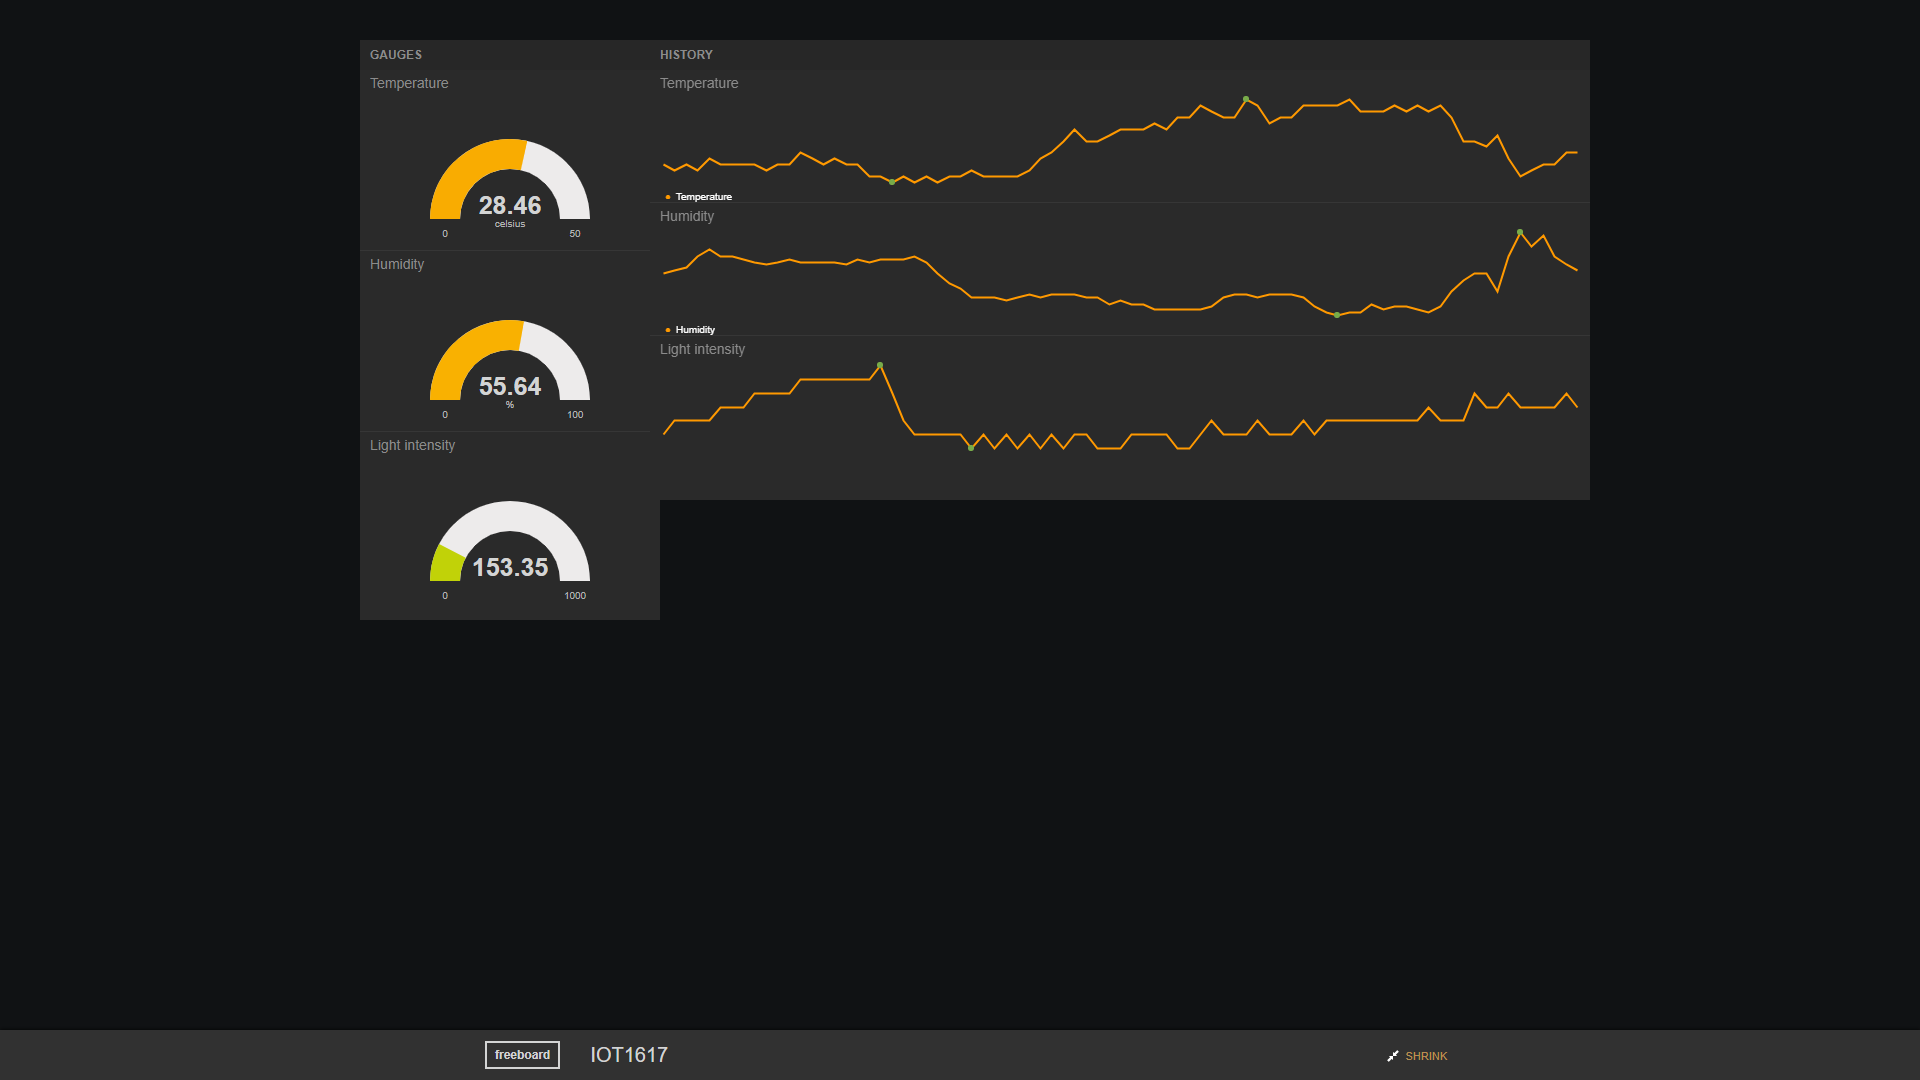
\includegraphics[width=\textwidth]{freeboard}
\caption{Freeboard.io dashboard}
\label{fig:freeboard}
\end{figure}

\begin{figure}
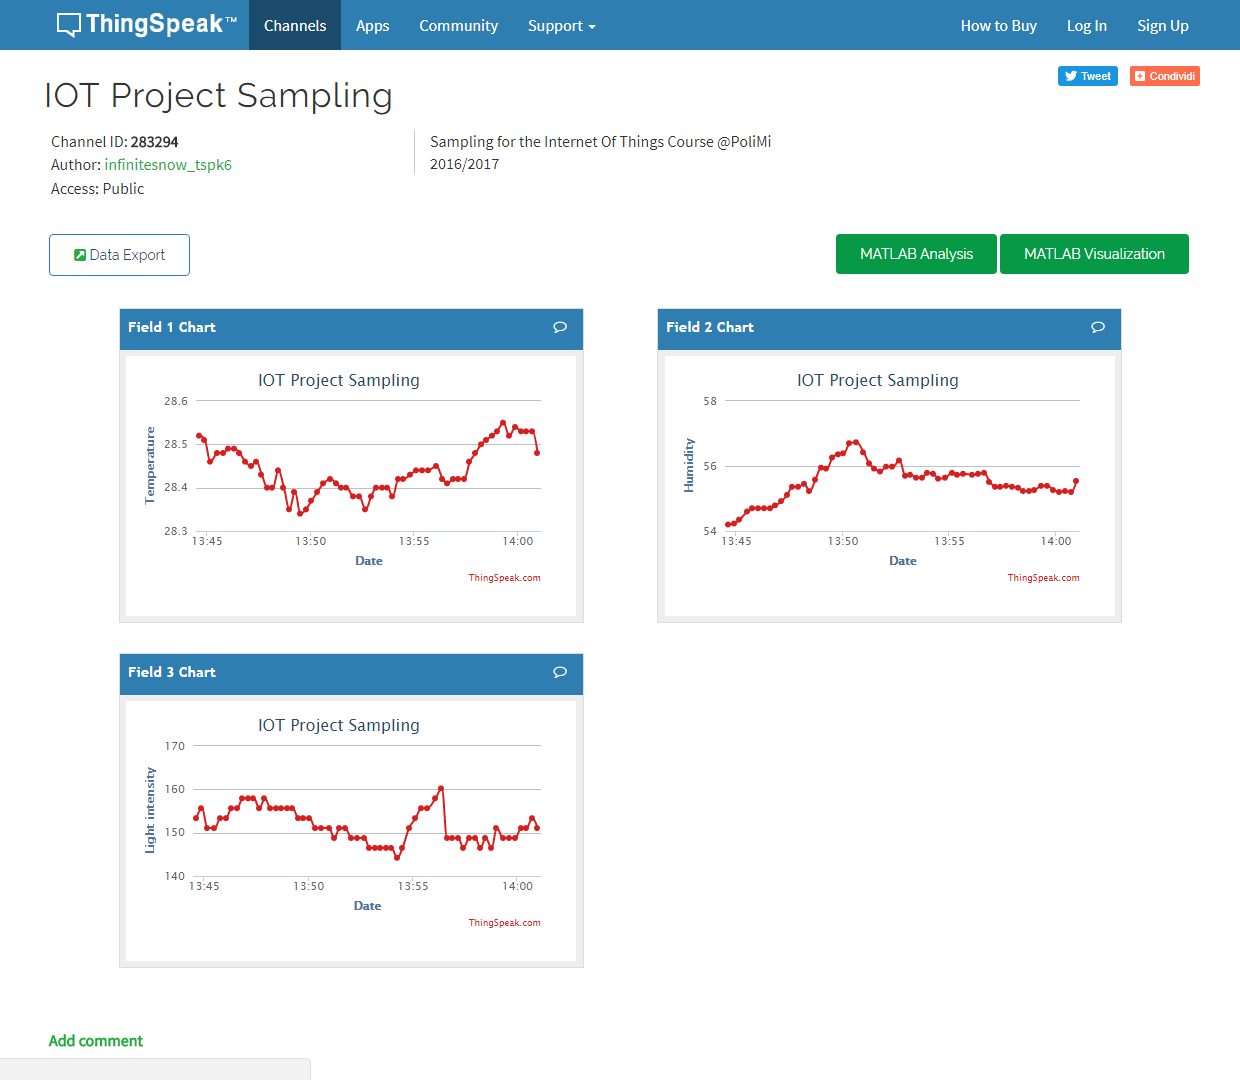
\includegraphics[width=\textwidth]{thingspeak}
\caption{Thingspeak channel}
\label{fig:thingspeak}
\end{figure}

\section{Reading the serial port}
Instead of using \texttt{node-red}'s integrated serial module, I decided to manually create a script to read from the serial port using Python's \texttt{Serial} module. This is the relevant part of the code, which parses the packet. 

\begin{lstlisting}
struct.unpack_from('>IIIHH',data_raw,2)
\end{lstlisting}

The relevant part of our payload is a 32 bit unsigned integer counter, and two 16 bit unsigned integer sensor readings. The first 64 bits are the package header, and are ignored. Data is shifted 16 bits to strip the footer off. Notice the \texttt{>} at the beginning of the format. This tells Python that packages use big endian numbers.

\section{Sensor calibration}
The only sensor I needed to use was a Sensirion SHT11, which provided humidity and temperature readings. I picket the transfer function coefficients from the vendor datasheet. For the humidity, we have:
$$\text{humidity}=c_1+c_2\cdot x +c_3\cdot x^2$$
where
$$c_1= -2.0468$$
$$c_2=  0.0367$$
$$c_3= -1.5955\cdot10^{-6}$$
for the temperature, we have
$$\text{temperature}=d_1+d_2\cdot x$$ 
$$d_1= -40$$
$$d_2=  0.01$$

\section{Filtering the serial readings}
The input data was not clean, and had to be filtered. At regular intervals, some packets didn't have the expected contents. I chose to filter them downstream of the publishing, because I wanted to keep track of them somehow. 

\begin{figure}
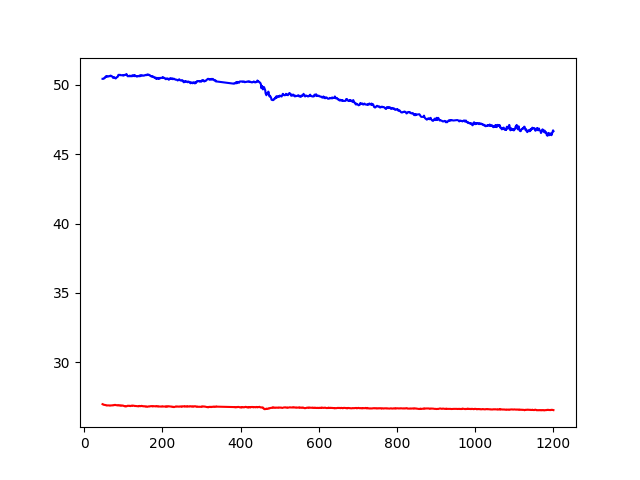
\includegraphics[width=\textwidth]{log-201756}
\end{figure}

\begin{figure}
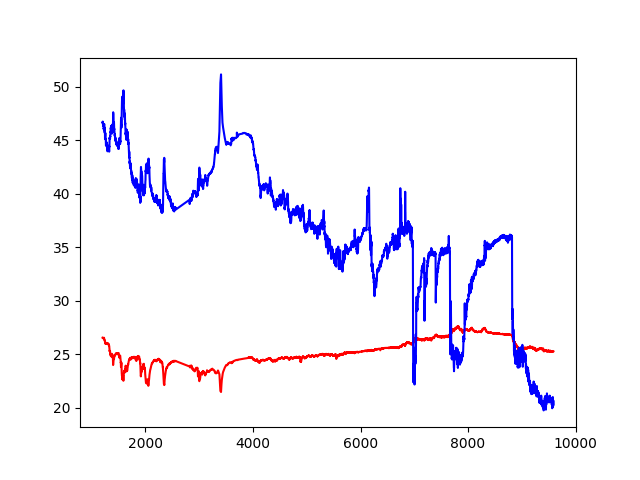
\includegraphics[width=\textwidth]{log-201757}
\end{figure}

\begin{figure}
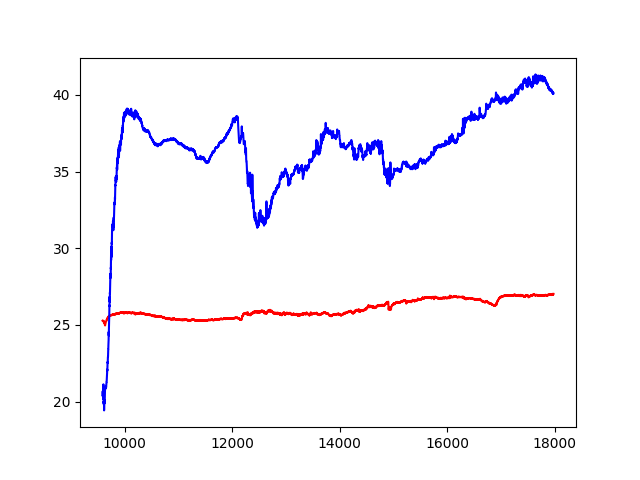
\includegraphics[width=\textwidth]{log-201758}
\end{figure}

\begin{figure}
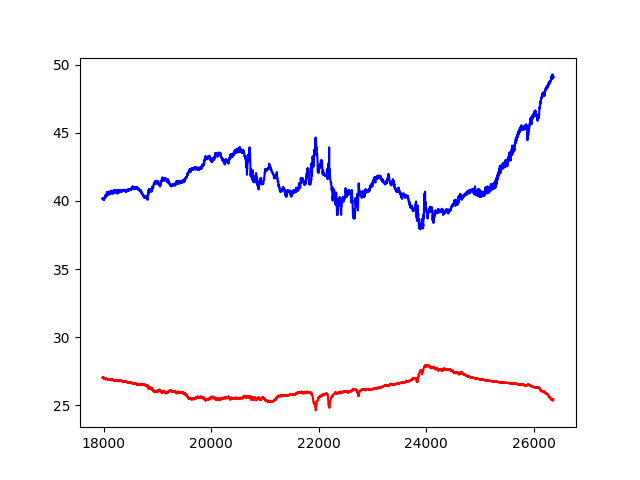
\includegraphics[width=\textwidth]{log-201759}
\end{figure}

\end{document}
